% warplane-proposal.tex — infraBUIDL() Grant Proposal & Press Kit
% Compile with: xelatex warplane-proposal.tex (run twice for TOC)

\documentclass[11pt,a4paper]{article}

% ── Fonts ──
\usepackage{fontspec}
\setmainfont{Helvetica Neue}[
  BoldFont = {Helvetica Neue Bold},
  ItalicFont = {Helvetica Neue Italic},
]
\setsansfont{Helvetica Neue}
\setmonofont{Menlo}[Scale=0.85]

% ── Layout ──
\usepackage[margin=2.5cm, top=3cm, bottom=3cm]{geometry}
\usepackage{parskip}
\usepackage{enumitem}
\setlist{nosep, leftmargin=1.5em}

% ── Colors ──
\usepackage{xcolor}
\definecolor{avaxred}{HTML}{E84142}
\definecolor{avaxdark}{HTML}{1A1A2E}
\definecolor{avaxgray}{HTML}{4A4A6A}
\definecolor{lightgray}{HTML}{F5F5FA}
\definecolor{accentblue}{HTML}{2563EB}
\definecolor{successgreen}{HTML}{059669}

% ── Tables ──
\usepackage{booktabs}
\usepackage{tabularx}
\usepackage{colortbl}
\usepackage{array}
\newcolumntype{L}[1]{>{\raggedright\arraybackslash}p{#1}}
\newcolumntype{C}[1]{>{\centering\arraybackslash}p{#1}}

% ── Graphics & Boxes ──
\usepackage{tikz}
\usetikzlibrary{calc, positioning, shapes.geometric, arrows.meta}
\usepackage{tcolorbox}
\tcbuselibrary{skins, breakable}

% ── Headers ──
\usepackage{titlesec}
\titleformat{\section}{\Large\bfseries\color{avaxdark}}{}{0em}{}[\vspace{-0.5em}\textcolor{avaxred}{\rule{\textwidth}{1.5pt}}]
\titleformat{\subsection}{\large\bfseries\color{avaxdark}}{}{0em}{}
\titleformat{\subsubsection}{\normalsize\bfseries\color{avaxgray}}{}{0em}{}

% ── Page Headers/Footers ──
\usepackage{fancyhdr}
\pagestyle{fancy}
\fancyhf{}
\renewcommand{\headrulewidth}{0pt}
\fancyhead[L]{\small\color{avaxgray}Warplane --- infraBUIDL() Proposal}
\fancyhead[R]{\small\color{avaxgray}April 2026}
\fancyfoot[C]{\small\color{avaxgray}\thepage}

% ── Hyperlinks ──
\usepackage{hyperref}
\hypersetup{
  colorlinks=true,
  linkcolor=avaxred,
  urlcolor=accentblue,
  pdfauthor={Warplane Project},
  pdftitle={Warplane: Interchain Control Plane for Avalanche L1s},
}

% ── Custom Boxes ──
\newtcolorbox{metricbox}[1][]{
  colback=lightgray,
  colframe=avaxred,
  fonttitle=\bfseries\color{white},
  coltitle=white,
  colbacktitle=avaxred,
  title=#1,
  boxrule=0pt,
  leftrule=3pt,
  arc=2pt,
  left=8pt, right=8pt, top=6pt, bottom=6pt,
}

\newtcolorbox{highlightbox}{
  colback=avaxred!5,
  colframe=avaxred,
  boxrule=0pt,
  leftrule=4pt,
  arc=0pt,
  left=10pt, right=10pt, top=8pt, bottom=8pt,
}

\newtcolorbox{gapbox}{
  colback=avaxdark!5,
  colframe=avaxdark,
  boxrule=0pt,
  leftrule=4pt,
  arc=0pt,
  left=10pt, right=10pt, top=8pt, bottom=8pt,
}

% ══════════════════════════════════════════════════════════════════
\begin{document}

% ── COVER PAGE ──
\thispagestyle{empty}
\begin{tikzpicture}[remember picture, overlay]
  % Background
  \fill[avaxdark] (current page.south west) rectangle (current page.north east);
  % Red accent bar
  \fill[avaxred] ([yshift=-12cm]current page.north west) rectangle ([yshift=-12.4cm]current page.north east);
  % Title block
  \node[anchor=west, text=white, font=\fontsize{42}{50}\selectfont\bfseries]
    at ([xshift=2.5cm, yshift=-5cm]current page.north west) {WARPLANE};
  \node[anchor=west, text=avaxred, font=\fontsize{16}{20}\selectfont]
    at ([xshift=2.5cm, yshift=-7cm]current page.north west) {The Interchain Control Plane for Avalanche L1s};
  % Subtitle
  \node[anchor=west, text=white!70, font=\fontsize{12}{16}\selectfont]
    at ([xshift=2.5cm, yshift=-9cm]current page.north west) {infraBUIDL() Grant Proposal \& Technical Overview};
  \node[anchor=west, text=white!50, font=\fontsize{10}{14}\selectfont]
    at ([xshift=2.5cm, yshift=-10cm]current page.north west) {April 2026 \ | \ Version 1.0 \ | \ Apache-2.0 Open Source};
  % Stats bar at bottom
  \node[anchor=west, text=white!60, font=\fontsize{9}{12}\selectfont]
    at ([xshift=2.5cm, yshift=3cm]current page.south west)
    {81 Mainnet L1s \quad\textcolor{avaxred}{\textbullet}\quad Zero ICM Observability \quad\textcolor{avaxred}{\textbullet}\quad \$150K Grant Request \quad\textcolor{avaxred}{\textbullet}\quad 4 Milestones};
  % GitHub link
  \node[anchor=west, text=accentblue, font=\fontsize{9}{12}\selectfont]
    at ([xshift=2.5cm, yshift=1.8cm]current page.south west)
    {\href{https://github.com/merged-one/warplane}{github.com/merged-one/warplane}};
\end{tikzpicture}
\clearpage

% ── TABLE OF CONTENTS ──
\thispagestyle{empty}
\tableofcontents
\clearpage

% ══════════════════════════════════════════════════════════════════
\section{Executive Summary}

\begin{highlightbox}
\textbf{Avalanche has 81 mainnet L1s, hundreds more in development, and zero dedicated tooling for cross-chain message observability, policy enforcement, or automated remediation.} Warplane is the first and only open-source operations platform purpose-built for Avalanche ICM/Teleporter messaging.
\end{highlightbox}

\medskip

Warplane requests \textbf{\$150,000} from Avalanche's infraBUIDL() program to deliver a production-grade Interchain Control Plane across four milestones over 10 months. The platform transforms the current state---where operators debug cross-chain messages through manual RPC calls and raw log parsing---into a unified operations layer with real-time tracing, automated alerting, declarative policy enforcement, and one-click remediation workflows.

\textbf{Milestone~1 is already complete}: an open-source monorepo with a validated domain model mapping all 8 TeleporterMessenger contract events, a deterministic Go test harness producing 5 cross-chain scenarios, full CI, and a local web dashboard. Every line of code is Apache-2.0 licensed.

\begin{metricbox}[Key Numbers]
\begin{tabularx}{\textwidth}{@{}X X X X@{}}
\textbf{81+} & \textbf{0} & \textbf{11} & \textbf{60s} \\
Mainnet L1s & Existing ICM tools & Event lifecycle kinds & Zero-to-traced \\
\end{tabularx}
\end{metricbox}

% ══════════════════════════════════════════════════════════════════
\section{The Problem}

\subsection{A Critical Gap in the Avalanche Ecosystem}

Avalanche's Interchain Messaging (ICM) protocol, built on Teleporter and AWM (Avalanche Warp Messaging), enables arbitrary cross-chain communication between L1s. With Avalanche9000 (ACP-77) reducing L1 creation costs by \textbf{99.9\%}, the number of L1s is accelerating rapidly.

But the operations tooling has not kept pace:

\begin{gapbox}
\textbf{No cross-chain message explorer exists for Avalanche ICM.}\\
\textbf{No relayer health dashboard exists.}\\
\textbf{No automated alerting for stuck or failed messages exists.}\\
\textbf{No policy enforcement for cross-chain messaging exists.}\\
\textbf{No remediation workflows (retry, fee top-up) exist.}\\[4pt]
Every other major cross-chain protocol has at least a read-only explorer. Avalanche ICM has \emph{nothing}.
\end{gapbox}

\subsection{Evidence of Pain}

The demand is not theoretical. These are open issues on Ava Labs' own repositories:

\begin{table}[h]
\centering
\small
\begin{tabularx}{\textwidth}{@{}l L{10cm}@{}}
\toprule
\textbf{Issue} & \textbf{Description} \\
\midrule
\href{https://github.com/ava-labs/avalanche-cli/issues/1616}{avalanche-cli \#1616} & Requests automatic trace/debug config for Teleporter subnets \\
\href{https://github.com/ava-labs/icm-services/issues/1066}{icm-services \#1066} & Most common relayer restart cause (block header race) with no monitoring \\
\href{https://github.com/ava-labs/icm-services/issues/695}{icm-services \#695} & Signature aggregator returns opaque errors; operators cannot diagnose \\
\href{https://github.com/ava-labs/icm-services/issues/473}{icm-services \#473} & Failed transactions not retried; recovery only on full relayer restart \\
\href{https://github.com/ava-labs/icm-services/issues/720}{icm-services \#720} & Relayer fatally errors on connection failure instead of graceful degradation \\
\href{https://github.com/ava-labs/icm-services/issues/602}{icm-services \#602} & Health check kills the relayer instead of allowing orchestrator recovery \\
\bottomrule
\end{tabularx}
\end{table}

\subsection{The Operational Complexity Scales Quadratically}

With $N$ L1s, the number of potential cross-chain messaging pairs is $\frac{N(N-1)}{2}$. Each pair requires independent relayer configuration, validator set tracking, and RPC endpoint management. At 81 L1s, that is \textbf{3,240 potential route pairs}---each one a potential failure point with no visibility.

% ══════════════════════════════════════════════════════════════════
\section{Market Analysis}

\subsection{Cross-Chain Message Explorers}

Every major cross-chain protocol has a dedicated explorer---except Avalanche ICM.

\begin{table}[h]
\centering
\small
\begin{tabularx}{\textwidth}{@{}l l C{1.5cm} C{2cm} C{2.5cm}@{}}
\toprule
\textbf{Explorer} & \textbf{Protocol} & \textbf{Chains} & \textbf{Operations} & \textbf{Remediation} \\
\midrule
WormholeScan & Wormhole & 25+ & None & None \\
LayerZero Scan & LayerZero V2 & 100+ & None & None \\
Axelarscan & Axelar GMP & 70+ & None & Manual retry \\
Hyperlane Explorer & Hyperlane & EVM & None & None \\
CCIP Explorer & Chainlink & 60+ & None & None \\
Range Security & Multi & 300+ & Alerts & None \\
\rowcolor{avaxred!10}
\textbf{Avalanche ICM} & \textbf{AWM/Teleporter} & \textbf{81+} & \textbf{None} & \textbf{None} \\
\bottomrule
\end{tabularx}
\caption{Cross-chain explorer comparison. Avalanche ICM is the only major protocol with zero dedicated tooling.}
\end{table}

\subsection{Blockchain Operations Platforms}

All major operations platforms are single-chain-scoped with no cross-chain message lifecycle awareness.

\begin{table}[h]
\centering
\small
\begin{tabularx}{\textwidth}{@{}l L{5cm} C{2cm} C{2cm}@{}}
\toprule
\textbf{Platform} & \textbf{Scope} & \textbf{Cross-chain} & \textbf{Open Source} \\
\midrule
Tenderly & Full-stack ChainOps & No & CLI only \\
Alchemy Notify & Event webhooks & No & No \\
QuickNode Streams & Data ingestion & No & No \\
OpenZeppelin Defender & Contract ops & Single-chain & No \\
Forta Network & Threat detection & Per-chain & Partially \\
\bottomrule
\end{tabularx}
\caption{No platform tracks cross-chain message lifecycles. None is open source.}
\end{table}

\subsection{Whitespace Map}

\begin{table}[h]
\centering
\small
\begin{tabularx}{\textwidth}{@{}L{7cm} C{3cm} C{3cm}@{}}
\toprule
\textbf{Capability} & \textbf{Industry} & \textbf{Avalanche} \\
\midrule
Cross-chain message viewing & Protocol-locked & \textcolor{avaxred}{\textbf{Nothing}} \\
Message lifecycle indexing & No native support & \textcolor{avaxred}{\textbf{Nothing}} \\
Cross-chain alerting & None & \textcolor{avaxred}{\textbf{Nothing}} \\
Policy enforcement & Complete whitespace & \textcolor{avaxred}{\textbf{Nothing}} \\
Automated remediation & Manual retry only & \textcolor{avaxred}{\textbf{Nothing}} \\
SLA monitoring & Complete whitespace & \textcolor{avaxred}{\textbf{Nothing}} \\
Environment promotion & Complete whitespace & \textcolor{avaxred}{\textbf{Nothing}} \\
Open-source cross-chain ops & Does not exist & \textcolor{avaxred}{\textbf{Nothing}} \\
\bottomrule
\end{tabularx}
\caption{Whitespace analysis. Every cell in the Avalanche column represents an opportunity Warplane addresses.}
\end{table}

% ══════════════════════════════════════════════════════════════════
\section{The Solution: Warplane}

\begin{highlightbox}
\textbf{Warplane} is an open-source Interchain Control Plane that gives Avalanche L1 operators complete visibility into cross-chain message lifecycles, with policy enforcement and automated remediation that no other tool---on any chain---provides.
\end{highlightbox}

\subsection{What Warplane Delivers}

\begin{enumerate}[label=\textcolor{avaxred}{\arabic*.}]
  \item \textbf{Per-message tracing} across source and destination L1s, correlating on-chain events with off-chain relay and signature aggregation
  \item \textbf{Relayer operations dashboard} with health metrics, latency tracking, and failure classification
  \item \textbf{Webhook alerting} for configurable conditions (stuck messages, high latency, relayer failures)
  \item \textbf{Declarative policy engine} enforcing operational constraints: allowed relayers, fee floors, retry windows, route allowlists, and circuit breakers
  \item \textbf{One-click remediation} for common failure modes: retry failed messages, top up fees, pause unhealthy routes, failover relayers
  \item \textbf{Environment promotion} pipeline from local development to Fuji testnet to mainnet
\end{enumerate}

\subsection{Target Users}

\begin{table}[h]
\centering
\small
\begin{tabularx}{\textwidth}{@{}l L{10cm}@{}}
\toprule
\textbf{Persona} & \textbf{Value Proposition} \\
\midrule
L1 Operator & Real-time visibility into ICM message health, automated alerting, remediation \\
Cross-chain dApp Developer & Debug message failures in minutes instead of hours, test locally with fixtures \\
Platform / DevOps Team & Multi-chain governance, policy enforcement, SLA monitoring, audit logging \\
Relayer Operator & Health dashboard, failure classification, latency benchmarks, auto-recovery \\
\bottomrule
\end{tabularx}
\end{table}

% ══════════════════════════════════════════════════════════════════
\section{Technical Architecture}

\subsection{11-Event Lifecycle Model}

Warplane's domain model maps the complete Teleporter message lifecycle. The TeleporterMessenger contract (v1.0.9) emits exactly 8 Solidity events. Warplane extends this with 3 off-chain derived events that capture the relay and aggregation phases invisible on-chain.

\begin{table}[h]
\centering
\small
\begin{tabularx}{\textwidth}{@{}l C{1.5cm} L{5cm} l@{}}
\toprule
\textbf{Warplane Event} & \textbf{Source} & \textbf{Contract Event} & \textbf{Chain} \\
\midrule
\texttt{message\_sent} & On-chain & \texttt{SendCrossChainMessage} & Source \\
\texttt{warp\_message\_extracted} & Off-chain & Relayer observes Warp log & Source \\
\texttt{signatures\_aggregated} & Off-chain & BLS aggregation completes & Off-chain \\
\texttt{relay\_submitted} & Off-chain & Relayer submits delivery tx & Destination \\
\texttt{delivery\_confirmed} & On-chain & \texttt{ReceiveCrossChainMessage} & Destination \\
\texttt{execution\_failed} & On-chain & \texttt{MessageExecutionFailed} & Destination \\
\texttt{retry\_requested} & On-chain & \texttt{retryMessageExecution} call & Destination \\
\texttt{retry\_succeeded} & On-chain & \texttt{MessageExecuted} (retry) & Destination \\
\texttt{fee\_added} & On-chain & \texttt{AddFeeAmount} & Source \\
\texttt{receipts\_sent} & On-chain & \texttt{ReceiptReceived} & Source \\
\texttt{replay\_blocked} & On-chain & Duplicate message ID rejected & Destination \\
\bottomrule
\end{tabularx}
\caption{Complete event-to-contract mapping. The 3 off-chain events provide the operational visibility that makes Warplane a control plane, not just an explorer.}
\end{table}

\subsection{Data Source Strategy}

\begin{metricbox}[Three Complementary Data Sources]
\begin{enumerate}[label=\textcolor{avaxred}{\arabic*.}, nosep]
  \item \textbf{RPC Polling} (\texttt{eth\_getLogs}) --- Primary source for all 8 TeleporterMessenger contract events. The only reliable method; AvaCloud Webhooks only support \texttt{address\_activity} and Glacier has no event-level indexing.
  \item \textbf{ICM Relayer Prometheus Metrics} (port 9090) --- 15 metrics including \texttt{successful\_relay\_message\_count}, \texttt{failed\_relay\_message\_count} (with \texttt{failure\_reason} label), \texttt{create\_signed\_message\_latency\_ms}, and \texttt{checkpoint\_committed\_height}.
  \item \textbf{Signature Aggregator Metrics} (port 8081) --- 11 metrics including \texttt{agg\_sigs\_latency\_ms}, \texttt{validator\_timeouts}, and \texttt{connected\_stake\_weight\_percentage}.
\end{enumerate}
\end{metricbox}

\subsection{Schema System}

All domain types are defined once in Zod v4 and automatically produce:
\begin{itemize}
  \item TypeScript types for compile-time safety
  \item JSON Schema for external validation
  \item OpenAPI 3.1 specs for API documentation
\end{itemize}

This single-source approach eliminates schema drift between the API, CLI, and dashboard.

\subsection{Architecture Diagram}

\begin{center}
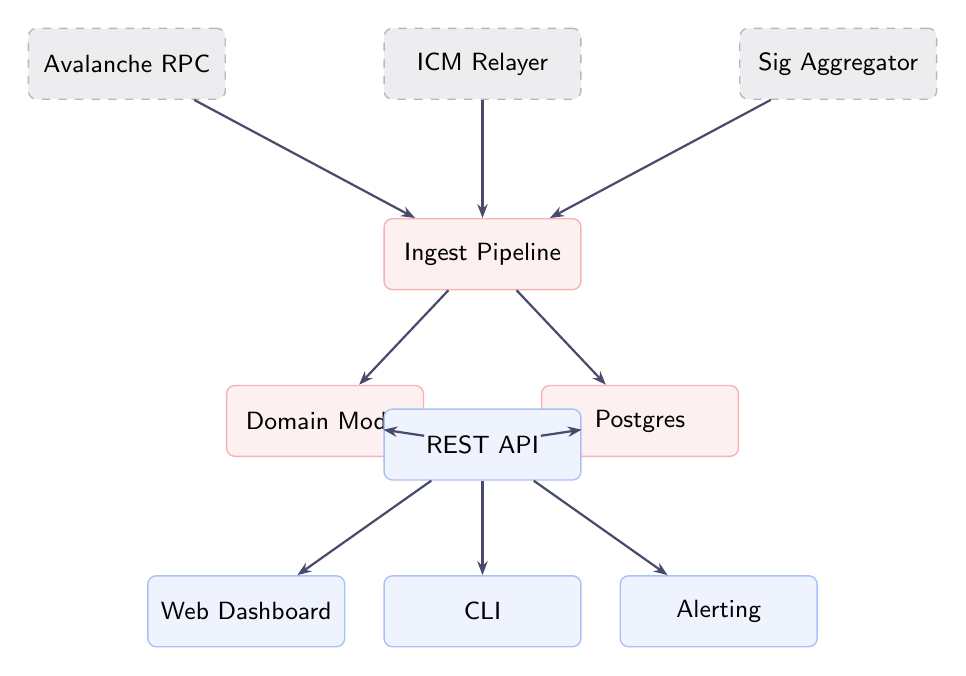
\begin{tikzpicture}[
  node distance=1.2cm and 2cm,
  box/.style={draw, rounded corners=3pt, minimum height=0.9cm, minimum width=2.5cm, font=\small\sffamily, fill=white, line width=0.5pt},
  databox/.style={box, fill=avaxred!8, draw=avaxred!40},
  appbox/.style={box, fill=accentblue!8, draw=accentblue!40},
  extbox/.style={box, fill=avaxgray!10, draw=avaxgray!40, dashed},
  arr/.style={-{Stealth[length=5pt]}, thick, color=avaxgray},
]
  % External sources
  \node[extbox] (rpc) {Avalanche RPC};
  \node[extbox, right=of rpc] (relayer) {ICM Relayer};
  \node[extbox, right=of relayer] (sigagg) {Sig Aggregator};

  % Ingest layer
  \node[databox, below=1.5cm of relayer] (ingest) {Ingest Pipeline};

  % Domain + Storage
  \node[databox, below=of ingest, xshift=-2cm] (domain) {Domain Model};
  \node[databox, below=of ingest, xshift=2cm] (storage) {Postgres};

  % API
  \node[appbox, below=1.5cm of ingest] (api) {REST API};

  % Apps
  \node[appbox, below=of api, xshift=-3cm] (web) {Web Dashboard};
  \node[appbox, below=of api] (cli) {CLI};
  \node[appbox, below=of api, xshift=3cm] (alerts) {Alerting};

  % Arrows
  \draw[arr] (rpc) -- (ingest);
  \draw[arr] (relayer) -- (ingest);
  \draw[arr] (sigagg) -- (ingest);
  \draw[arr] (ingest) -- (domain);
  \draw[arr] (ingest) -- (storage);
  \draw[arr] (domain) -- (api);
  \draw[arr] (storage) -- (api);
  \draw[arr] (api) -- (web);
  \draw[arr] (api) -- (cli);
  \draw[arr] (api) -- (alerts);
\end{tikzpicture}
\end{center}

% ══════════════════════════════════════════════════════════════════
\section{Milestone Roadmap}

\begin{table}[h]
\centering
\small
\begin{tabularx}{\textwidth}{@{}C{0.6cm} L{4cm} L{5.5cm} C{1.2cm} C{1.8cm}@{}}
\toprule
\textbf{\#} & \textbf{Name} & \textbf{Key Deliverables} & \textbf{Ask} & \textbf{Target} \\
\midrule
\rowcolor{successgreen!10}
M1 & Core Control Plane \& Test Harness & Open-source monorepo, API, CLI, 5 scenarios, CI, dashboard & \$30K & \textcolor{successgreen}{\textbf{Complete}} \\
\addlinespace
M2 & Fuji Alpha: Observability \& Eventing & RPC ingestion, relayer/sig-agg metrics, tracing UI, alerting, Postgres, Docker Compose & \$40K & Aug 2026 \\
\addlinespace
M3 & Policy Engine \& Remediation & Declarative policies, retry/fee-top-up/circuit-breaker, env promotion, RBAC, audit log & \$35K & Nov 2026 \\
\addlinespace
M4 & Public Beta \& Ecosystem Launch & Security hardening, docs site, VRF reference integration, partner pilots, search & \$45K & Jan 2027 \\
\midrule
& & \textbf{Total} & \textbf{\$150K} & \\
\bottomrule
\end{tabularx}
\caption{Four milestones delivering incremental value. Each milestone produces a usable product, not just infrastructure.}
\end{table}

\subsection{Milestone 1: Complete}

\begin{metricbox}[M1 Achievements --- Verified in CI]
\begin{itemize}[nosep]
  \item 11-event domain model validated by Zod discriminated unions
  \item Go tmpnet test harness generating 5 deterministic cross-chain scenarios
  \item Golden fixture pipeline with CI validation on every commit
  \item REST API serving traces, networks, and chains
  \item CLI with JSON and TTY output modes
  \item Local React web dashboard for trace inspection
  \item 100\% CI pass rate --- zero-to-traced in $\sim$60 seconds
\end{itemize}
\end{metricbox}

\subsection{Why This Phasing}

\textbf{M1 $\rightarrow$ M2 (Observability First):} The research confirms observability is the most acute gap. Shipping a Fuji-connected alpha with real message tracing provides immediate value and validates the architecture before building policy layers.

\textbf{M2 $\rightarrow$ M3 (Policy \& Remediation):} Once observability proves the data model works with real Teleporter events, the policy engine enforces operational constraints that teams need for production. This transforms an explorer into a control plane.

\textbf{M3 $\rightarrow$ M4 (Beta \& Ecosystem Proof):} The final milestone validates the full stack with real users, a concrete reference integration (VRF cross-L1), and production-grade hardening.

% ══════════════════════════════════════════════════════════════════
\section{Why Now}

\subsection{Avalanche L1 Adoption Is Accelerating}

\begin{itemize}
  \item \textbf{81 mainnet L1s}, hundreds more in development
  \item \textbf{Avalanche9000 / ACP-77} reduced L1 creation cost by 99.9\%
  \item \textbf{Institutional adoption}: FIS Global (2,000 US banks), KBank, JP Morgan Evergreen
  \item \textbf{Transaction volume}: 1.45B total (+153\% YoY), 4.17M average daily
\end{itemize}

\subsection{ICM Infrastructure Is Maturing, Operations Tooling Is Not}

\begin{itemize}
  \item TeleporterMessenger at v1.0.9, ICM Relayer at v1.7.4
  \item Granite upgrade (Nov 2025) added epoched P-Chain validator views for ICM
  \item TeleporterMessengerV2 planned with multi-verification support
  \item But relayer stability issues remain (6+ open GitHub issues)
\end{itemize}

\subsection{No Competitor Is Building This}

\begin{itemize}
  \item No infraBUIDL or Retro9000 grantee has proposed ICM observability
  \item No GitHub project addresses this gap
  \item The closest analog (Range Security) focuses on security forensics, not DevOps
\end{itemize}

% ══════════════════════════════════════════════════════════════════
\section{Competitive Moat}

\begin{table}[h]
\centering
\small
\begin{tabularx}{\textwidth}{@{}l L{10cm}@{}}
\toprule
\textbf{Moat Factor} & \textbf{Detail} \\
\midrule
First mover & Only ICM/Teleporter operations tool in the ecosystem \\
Event model depth & 11-event lifecycle mapped to all 8 contract events + 3 off-chain states \\
Data source integration & RPC + relayer Prometheus (15 metrics) + sig-agg Prometheus (11 metrics) \\
Test harness & Deterministic Go tmpnet harness with 5 scenarios and golden fixtures \\
Open source & Apache-2.0 removes adoption friction; no OSS cross-chain ops tool exists \\
Schema system & Zod v4 single source producing TS types, JSON Schema, and OpenAPI 3.1 \\
Grant alignment & Hits 3 infraBUIDL categories: interoperability tools, explorers, indexers \\
\bottomrule
\end{tabularx}
\caption{Defensibility through depth of integration, not breadth of features.}
\end{table}

% ══════════════════════════════════════════════════════════════════
\section{Grant Budget}

\begin{table}[h]
\centering
\begin{tabularx}{\textwidth}{@{}C{1cm} L{5cm} C{2cm} L{5cm}@{}}
\toprule
\textbf{\#} & \textbf{Milestone} & \textbf{Amount} & \textbf{Primary Spend} \\
\midrule
M1 & Core Control Plane & \$30,000 & Development, CI infrastructure, testing \\
M2 & Fuji Alpha & \$40,000 & RPC infrastructure, Fuji deployment, Postgres \\
M3 & Policy Engine & \$35,000 & Development, security review \\
M4 & Public Beta & \$45,000 & Security audit, docs, partner onboarding \\
\midrule
& \textbf{Total} & \textbf{\$150,000} & \\
\bottomrule
\end{tabularx}
\end{table}

The budget assumes single-developer execution with potential contractor support for security auditing (M4) and design work (M2 dashboard). The \$150K total is modest for the 10-month scope but achievable given M1's demonstrated execution velocity.

% ══════════════════════════════════════════════════════════════════
\section{Forward Compatibility}

Warplane's architecture is designed to grow with the Avalanche ecosystem:

\begin{itemize}
  \item \textbf{TeleporterMessengerV2}: The 3 off-chain events (\texttt{warp\_message\_extracted}, \texttt{signatures\_aggregated}, \texttt{relay\_submitted}) will generalize to verification-scheme-agnostic labels when V2 adds multiple verification mechanisms beyond AWM
  \item \textbf{L1 growth}: The ingest pipeline scales horizontally---add new L1 RPC endpoints as configuration, not code changes
  \item \textbf{Retro9000}: Ecosystem impact from Warplane creates eligibility for retroactive grants based on adoption metrics
\end{itemize}

% ══════════════════════════════════════════════════════════════════
\section{Team \& Execution}

\begin{highlightbox}
\textit{[Team information to be completed by the applicant. Include background, relevant experience, and roles.]}
\end{highlightbox}

\textbf{Execution evidence:} Milestone~1 was completed in under 2 weeks, delivering a validated domain model, 5 test scenarios, full CI, and a web dashboard. The \href{https://github.com/merged-one/warplane}{open-source repository} demonstrates the team's ability to ship production-quality infrastructure at pace.

% ══════════════════════════════════════════════════════════════════
\section{Call to Action}

\begin{center}
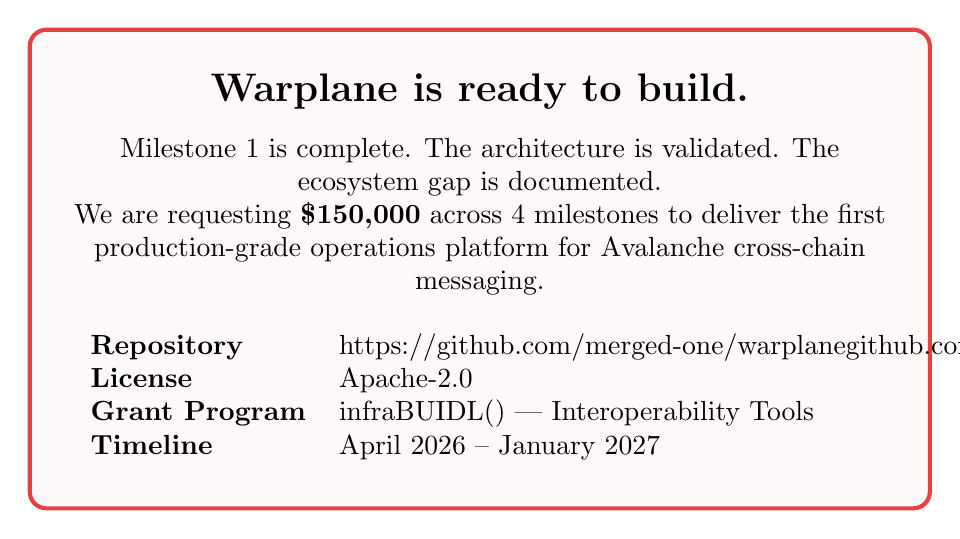
\begin{tikzpicture}
\node[draw=avaxred, line width=1.5pt, rounded corners=6pt, inner sep=16pt, fill=avaxred!3] {
\begin{minipage}{0.85\textwidth}
\centering
\textbf{\Large Warplane is ready to build.}\\[8pt]
\normalsize
Milestone~1 is complete. The architecture is validated. The ecosystem gap is documented.\\
We are requesting \textbf{\$150,000} across 4 milestones to deliver the first\\
production-grade operations platform for Avalanche cross-chain messaging.\\[12pt]
\begin{tabular}{l l}
\textbf{Repository} & \href{https://github.com/merged-one/warplane}{github.com/merged-one/warplane} \\
\textbf{License} & Apache-2.0 \\
\textbf{Grant Program} & infraBUIDL() --- Interoperability Tools \\
\textbf{Timeline} & April 2026 -- January 2027 \\
\end{tabular}
\end{minipage}
};
\end{tikzpicture}
\end{center}

\vfill

\begin{center}
\small\color{avaxgray}
\textit{81 mainnet L1s. Zero observability tooling. Until now.}
\end{center}

\end{document}
